\begin{figure}[h]
    \centering
    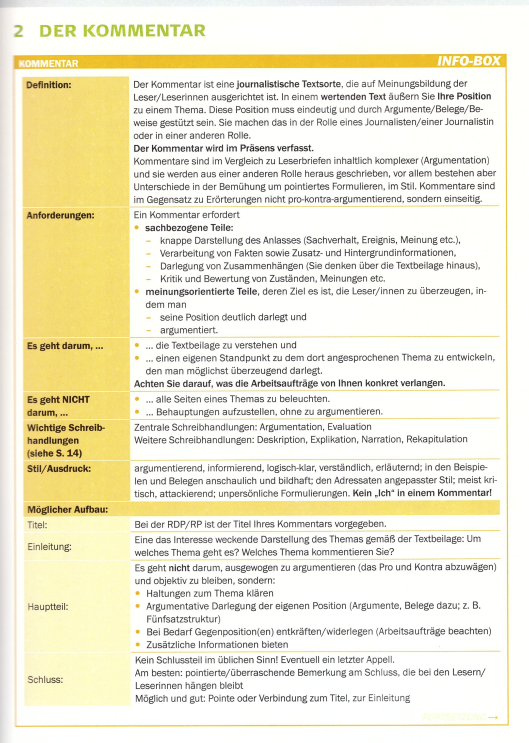
\includegraphics[scale=0.8]{./pics/Screenshot from 2023-02-06 12-27-40.png}
    \caption{Kommentar: Definition + Aufbau}
    \label{fig:impl:Kommentar1}
\end{figure}

\begin{figure}[h]
    \centering
    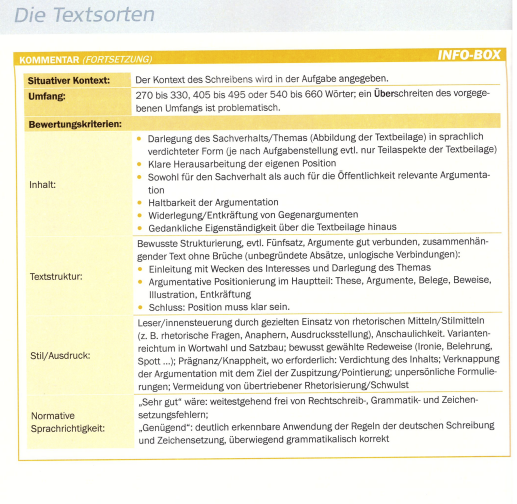
\includegraphics[scale=0.8]{./pics/Screenshot from 2023-02-06 12-27-54.png}
    \caption{Kommentar: Verfassen}
    \label{fig:impl:Kommentar2}
\end{figure}
\begin{figure}[h]
    \centering
    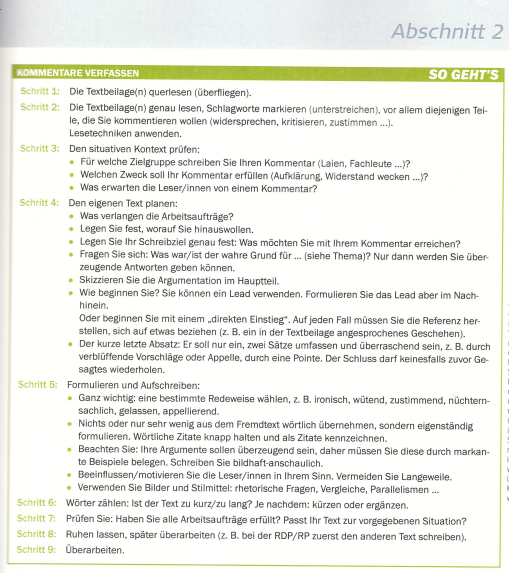
\includegraphics[scale=0.8]{./pics/Screenshot from 2023-02-06 12-28-08.png}
    \caption{Kommentar: Fortsetzung}
    \label{fig:impl:Kommentar3}
\end{figure}


\section{Mustertext}

\subsubsection{Man muss nicht alles haben}

Wahrscheinlich sind nicht alle Leser mit obigem Titel einverstanden. Es gibt zwar viele Einsichtige, die von der Notwendigkeit nachhaltigen Konsums überzeugt sind, aber leider auch viele Andersdenkende, die recht bedenkenlos das Luxusleben der Wegwerfgesellschaft genießen. 

Diese Haltung ärgert Sepp Eisenriegler, der sich als Präsident des Dachverbands für Sozialwirtschaft unermüdlich für soziale und ökologische Aspekte der Nachhaltigkeit und gegen unnötige Vernichtung wertvoller Ressourcen einsetzt. Er versucht die Menschen zu überzeugen, dass die Konsumgier nur dazu treibe, „immer mehr zu arbeiten, um immer mehr Besitztümer anzuhäufen, die man dann gar nicht genießen kann.“ 

 

In diese Falle tappen auch viele junge Menschen, wenn sie über ausreichend Taschengeld verfügen oder mit ihrem ersten selbstverdienten Geld sofort alles kaufen wollen, was als sogenanntes „Must-have“ beworben wird. Man sollte sie von etwas Besserem überzeugen! Aber wie? 

Die Wirkung eines guten Vorbilds gilt als bestes Erziehungsmittel; ein schlechtes bewirkt das Gegenteil. In einer Familie, in der jedes Haushaltsgerät schon beim kleinsten Schaden ohne Reparaturversuch sofort entsorgt und durch ein Neugerät ersetzt wird, wo der Vater alljährlich auf das neueste Automodell umsteigt und die Mutter sich jedem Modediktat beugt, wird auch der Nachwuchs kaum vom aktuellen Dringendwunsch abgebracht und vom Sinn des Sparens überzeugt werden können.  

Doch der Hebel muss auch noch woanders angesetzt werden, nämlich bei der Stärkung eines positiven Selbstbewusstseins. Tatsächlich ist es in der Pubertät oft ziemlich schwer, die eigene Meinung Andersdenkenden gegenüber zu vertreten. Doch mit ein bisschen Mut kann man seinen schon älteren Pullover als „Lieblingskleidung“ verteidigen und es nicht zulassen, dass die persönliche Akzeptanz in der Gruppe vom Besitz aller technischen Neuheiten abhängt. 

 

Erfreulicherweise behaupten viele junge Menschen, theoretisch ein „grünes Herz“ zu besitzen. Doch Worte allein genügen nicht - man muss auch Taten folgen lassen! Bekennt euch deshalb zu der Meinung, dass etwas Gebrauchtes nicht automatisch unbrauchbar ist und dass man nicht alles haben muss, um glücklich zu sein! 

 

313 Wörter 
\section{Eigener Text}

\subsubsection{Werden dicke Menschen dumm? }
In dem Bericht “Fettreiche Ernährung bremst Hirnreifung” geht es um eine Studie, welche die Auswirkungen von fettigem Essen auf Ratten untersucht. Dabei kam ans Licht, das durch zu viel Fett Ablagerung in gewissen Gehirnbereichen entstehen können, welche die Hirnreifung ausbremst. Da der Aufbau von der Ratte dem Menschlichen ähnelt, gab es für die Wissenschaftler Grund zur Sorge. Aus diesem Grund befasse ich mich hier in dem Kommentar, wie man den Konsum von fettreichem Essen vor allem bei Kindern und jungen Erwachsenen bremsen kann. 

 

Als erstes sind die Eltern eines Kindes dafür verantwortlich, was jene in den jungen Jahren zu sich nehmen. Doch viele Eltern möchten ihre Kinder verwöhnen, diese belohnen oder essen selbst gerne ungesundes Essen. Dadurch gewöhnen sich auch die jüngere Generation schnell an das beliebte fast food. Doch wie kann man das verhindern? In meinen Augen sind die Eltern selbst oft nicht gut genug aufgeklärt, was ungesundes Essen alles für negative Auswirkungen auf den menschlichen Körper haben kann. 

 

 Deswegen sollte man schon in den frühen Jahren in der Schule unterrichtet werden, wie man sich und den Körper gesund ernährt, wie man richtig Sport macht und was gesund für einen ist und was nicht. Außerdem würde ich es begrüßen, wenn es für Eltern, die gerade ihr erstes Kind erwarten, Fortbildungen gibt, wie sie ihr Kind richtig ernähren müssen. 

 

Aber natürlich ernähren sich Kinder nicht nur zu Hause bei ihren Eltern. Auch das Essen in der Schule selbst spielt eine wichtige Rolle. Deswegen ist es wichtig, ein anständiges und vor allem gesundes Essen für die Pausen bereitzustellen. In den meisten Schulen gibt es schon Buffets mit reichlich Auswahl, jedoch kommen gesunde und vor allem günstige Menüs immer zu kurz. In den meisten Schulen bekommt man belegte Brötchen oder andere kalte Speisen, aber warme Menüs oder spezielles Essen für Veganer und Vegetarier kommt immer zu kurz. Außerdem sollte das Angebot von ungesunden Essen wie zum Beispiel Pizza oder anderes Fast Food drastisch gesenkt werden. Eine Lösung wäre eine einheitliche Institution, die sich ausschließlich um das Essens-Angebot in Schulen kümmert. Zwar sind schon viele Buffets einer bestimmten Firma, jedoch gibt es da noch immer keine einheitlichen Regeln. 

Mein Appel an die Eltern und vor allem an die Politik: Unterschätzt die Folgen der ungesunden Ernährung bitte nicht. Sorgt für euch und eure Kinder. Und bitte klärt auf, wenn jemand darüber nicht Bescheid weiß! 

Ca 400 Wörter 

\newpage

\section{Formulierungshilfen}
\subsubsection{Einbinden von Informationen }
\begin{compactitem}
    \item "Der/Die Journalist*in XY vertritt in seinem/ihrem Artikel die Meinung, dass..." 
    \item "In dem Artikel XY aus der Tageszeitung XY wird dargestellt..." 
    \item "Das Interview mit dem Forscher XY verdeutlicht..." 
    \item "Eine Umfrage von XY hat ergeben.../...liefert interessante Ergebnisse zum Thema..." 
\end{compactitem}
\subsubsection{Verbinden von Argumenten oder Informationen }
Da Du einen Fließtext verfasst, in dem Du viele Informationen miteinander verknüpfst, sollte diese Verbindung auch sprachlich gekennzeichnet werden. Beispielsweise durch Satzanfänge wie: 
\begin{compactitem}
    \item "Außerdem ..." / "Zudem ..." / "Des Weiteren ..." / "Darüber hinaus ..." / "Folglich ..." / "Demzufolge ..." 
\end{compactitem}
Wenn Du dabei bist, die Gegenargumente zu widerlegen, eignen sich Formulierungen wie: 
\begin{compactitem}
    \item "Allerdings..."/"Jedoch.."/"Aber..."/"Trotzdem..
    \item "Dagegen lässt sich allerdings argumentieren..." 
    \item "Dem gegenüber steht jedoch das Argument..." 
    \item "Trotzdem muss man sagen..." 
    \item "Widerlegen lässt sich diese Behauptung damit, dass..." 
    \item  "Man kann zwar argumentieren, dass... , jedoch/allerdings/aber..."
    \item "Obwohl/Wenngleich behauptet wird, dass... , muss betont werden, dass..."  
\end{compactitem}
\subsubsection{Überleitung zum Fazit }
\begin{compactitem}
    \item "Zusammenfassend kann man sagen..." 
    \item "Es wird deutlich..." 
    \item "Die Studien/Untersuchungen/Befragungen zeigen/ergeben eindeutig..." 
    \item "Anhand dieser Punkte zeigt sich also..." 
    \item "Es steht außer Frage, dass..." 
    \item "Wie sich erkennen lässt..." 
\end{compactitem}
\subsection{Realitätsbezug: }
Der Kommentar findet sich vor allem in der Zeitung wieder. Hier findet man oft Kommentare (oder Leserbriefe) zu aktuellen Themen. Weitere Beispiele wären in sozialen Medien, Onlineforen, Kundenbewertungen und viele mehr. 

\subsubsection{Beispiele für verwandte Textsorten}
Glosse, Leitartikel, Rezension, Kolumne, Leserbrief, Erörterung
\subsubsection{Abgrenzung} Ausgesprochen elaborierte Leserbriefe können einem Kommentar
ähnlich sein, weisen jedoch seltener die inhaltliche Komplexität
(Argumentation) eines Kommentars auf. Ähnlichkeiten zur Erörterung
im argumentativen Vorgehen stehen Unterschiede in der Präsentation der Argumente, in der Art der eigenen Positionierung und im Stil
gegenüber.
\subsubsection{Umfang}
270 bis 330, 405 bis 495 oder 540 bis 660 Wörter

\subsubsection{situativer Kontext}erforderlich